\newcommand{\Add}[1]{\textcolor{blue}{#1}}
%\renewcommand{\d}{\mathrm{d}}
%\renewcommand{\e}{\mathrm{e}}
%\renewcommand{\i}{\mathrm{i}}
\newcommand{\hyb}{\mathrm{hyb}}
\newcommand{\NR}{\mathrm{NR}}
\newcommand{\pN}{\mathrm{pN}}
\newcommand{\ADMMass}{M_{\mathrm{ADM}}}
\newcommand{\IrrMass}{M_{\mathrm{AH}}}
\newcommand{\MSun}{\ensuremath{M_{\odot}}}
\newcommand{\deff}{\ensuremath{D_{\mathrm{eff}}}} % effective distance
\newcommand{\ta}{\ensuremath{t_{\mathrm{a}}}}
\newcommand{\phia}{\ensuremath{\phi_{\mathrm{a}}}}
\newcommand{\fsamp}{\ensuremath{f_{\mathrm{s}}}}
\newcommand{\fNy}{\ensuremath{f_{\mathrm{Ny}}}}
\newcommand{\discretize}{\rightsquigarrow}
\newcommand{\software}[1]{\textsc{#1}}
\newcommand{\etal}{\textit{et al.}\xspace}
\newcommand{\G}{G}
\renewcommand{\c}{c}
\newcommand{\e}{e}
%\newcommand{\lvert}{\ensuremath{|}}
%\newcommand{\rvert}{\ensuremath{|}}

%%% Define \InnerProduct with extendible middle line
%%% Adapted from braket.sty
\makeatletter
\let\protect\relax
{\catcode`\|=\active
  \xdef\InnerProduct{\protect\expandafter\noexpand\csname InnerProduct \endcsname}
  \expandafter\gdef\csname InnerProduct \endcsname#1{%
    \begingroup
    \ifx\SavedDoubleVert\relax
    \let\SavedDoubleVert\|\let\|\IpDoubleVert
    \fi
    \mathcode`\|32768\let|\IPVert
    \left({#1}\right)
    \endgroup
  }
}
\def\IPVert{\@ifnextchar|{\|\@gobble}% turn || into \|
     {\egroup\,\mid@vertical\,\bgroup}}
\def\IPDoubleVert{\egroup\,\mid@dblvertical\,\bgroup}
\let\SavedDoubleVert\relax
\def\midvert{\egroup\mid\bgroup}
\def\SetVert{\@ifnextchar|{\|\@gobble}% turn || into \|
    {\egroup\;\mid@vertical\;\bgroup}}
\def\SetDoubleVert{\egroup\;\mid@dblvertical\;\bgroup}
\def\mid@vertical{\mskip1mu\vrule\mskip1mu}
\def\mid@dblvertical{\mskip1mu\vrule\mskip2.5mu\vrule\mskip1mu}
\makeatother


\Note{Numbers in this chapter are subject to change after 
completing the reruns to fix the sign error in the 
3pN term}

\section{Introduction}
\label{sec:Introduction} %

In chapter~\ref{ch:search} we outlined the CBC pipeline used to search
LIGO/Virgo data for gravitational waves resulting from the inspiral of
binary systems composed of neutron stars and/or black holes.  In
particular we noted the use of post-Newtonian templates of the form
discussed in section~\ref{sec:PNWaveforms} to filter the data up to a
total mass of $25 \msun$.  The post-Newtonian approximation is valid
so long as the velocities of the component masses are small compared
to the speed of light, or equivalently so long as the orbital
frequencies are small.  In current searches the waveform is terminated
at the Schwarzschild ISCO frequency after which the inspiral
transitions to a plunge, although this is only strictly correct in the
point-mass limit.

For systems containing two neutron stars this frequency is above 1000
Hz, even for a hypothetical system composed of two instances of the
heaviest-known neutron star.  This is well outside LIGO's most
sensitive band where most of the SNR will be accumulated, and we may
therefore trust pN waveforms for a BNS search.  However, for systems
including at least one black hole the ISCO frequency will be lower and
the merger may occur in the sensitive band.  It is therefore
important to test the ability of pN templates to detect such systems
and where possible optimize their use.  In order to evaluate the
effectiveness of templates it is necessary to compare them
against complete waveforms including the inspiral, merger and ringdown
phases.  This necessitates the use of hybrid pN-NR waveforms as
described in section~\ref{sec:HybridWaveforms}.  This chapter uses
high-accuracy waveforms developed at Caltech and Cornell~\footnote{The
code used to produce these waveforms, SpEC, is now being developed and
used by a collaboration including scientists at Caltech, Cornell and
the Canadian Institute for Theoretical Astrophysics (CITA).}. 

The most robust test would consider the ability of the full pipeline
to detect BBH signals; this is the goal of the NINJA project
introduced in the following chapter.  Here we focus on a more
fundamental question, the ability of pN waveforms to capture full
physical signals.  We test this by calculating the overlap (defined in
eqn.~\ref{eq:OverlapDefinition}) between the hybrid waveform and the
pN approximation.  If there are no parameters for which the chosen pN
model provides a high overlap with the hybrid signal then the pipeline
as a whole will be unable to detect such signals.  A similar study has
been performed by Pan~\etal using numerical data from Pretorius and
the Goddard groups~\cite{Pan2007}.  Our main results are in agreement
with their conclusion that a simple extension of the TaylorF2
waveforms currently in use by the CBC low-mass search yields high
overlaps with numerical waveforms.

Throughout this chapter we use only the $(l,m)=(2,2)$ component of the
waveform $\Psi_{4}^{2,2}$ (as defined, e.g., in~\cite{Boyle2008a}).
For convenience, we drop the superscript.  Whenever possible, we use
dimensionless quantities, like $r\,M\,\lvert \Psi_{4} \rvert$, where
$r$ is the areal radius of the observation sphere, and $M$ is the
total apparent-horizon mass of the holes in the initial data.
However, for any calculation involving the LIGO noise curve, we have a
physical scale, and thus use standard mks units.  

To weight the inner products in the overlap we use the
following PSDs for Initial and Advanced LIGO: for Initial LIGO we use
an analytic approximation to the LIGO design PSD given by
\begin{eqnarray}
  S_n(f) &= &3.136 \times 10^{-4} \bigg[
  \left(\frac{ 4.49 f}{150.0}\right)^{-56.0} \nonumber \\
  &+ & 0.16 \left(\frac{f}{150}\right)^{-4.52}
  + \left(\frac{f}{150.0}\right)^2 + 0.52
  \bigg]
\end{eqnarray}
All integrals start from 40 Hz.  As shown in
Fig.~\ref{fig:StildesAndInitialPSD}, at this frequency the noise is an
order of magnitude higher than its lowest value, and below this
frequency it rises rapidly as $\sim f^{-56}$.  The region below 40 Hz
therefore contributes very little signal power to the
SNR~\cite{Abbott:2007xi}.  

For Advanced LIGO we use the GWINC program~\cite{AdvancedLIGONoise} to
generate the PSD.  GWINC reports the PSD in increments of 0.0124 Hz.
When calculating discrete integrals against signals sampled at other
frequencies we obtain values for the PSD by linearly interpolating
between the values provided by GWINC.  We start integrals at 10 Hz as
that is the point where the noise has increased by two orders of
magnitude above its minimum, as also shown in
Fig.~\ref{fig:StildesAndInitialPSD}.




%%%%%%%%%%%%%%%%%%%%%%%%%%%%%%%%%%%%%%%%%%%%%%%%%%%%%%%%%%%%%%%%%%%%%%
%%%%%%%%%%%%%%%%%%%%%%%%%%%%%%%%%%%%%%%%%%%%%%%%%%%%%%%%%%%%%%%%%%%%%%
\section{PN--NR hybrid waveform}
\label{sec:PNNRHybridWaveform} %


In order to perform our comparison we need to construct a ``true''
black-hole binary waveform, which we might expect to observe with
detectors.  A numerical simulation provides the data for the crucial
nonlinear merger phase.  We carefully extract the data and extrapolate
it to large radius, and investigate the effects of numerical error on
the final result.  Because this waveform is very computationally
expensive to produce, it covers only about 32 cycles, which is not
sufficient for a thorough investigation of the possibility of
detecting it in searches of data from gravitational-wave detectors.
Thus, we match the numerical waveform to a post-Newtonian waveform,
producing a hybrid which extends for many thousands of cycles,
covering the entire band of interest.

\subsection{Numerical simulation, extraction, and extrapolation}
\label{sec:WaveformExtractionAndExtrapolation}
The numerical simulation is the same as that described in
Refs.~\cite{Boyle2007, Scheel2008}: an equal-mass, non-spinning,
black-hole binary with reduced
eccentricity~\cite{Pfeiffer-Brown-etal:2007}, beginning roughly 16
orbits before merger, continuing through merger and
ringdown~\cite{Scheel2008}.  It is performed with the Caltech--Cornell
pseudospectral code, using boundary conditions designed to prevent
constraint violations and gravitational radiation from entering the
domain~\cite{Holst2004, Lindblom2006}.

Data is extracted from the simulation in the form of the
Newman--Penrose scalar
\begin{equation}
  \Psi_{4} = -C_{\alpha \beta \gamma \delta} l^{\alpha}
  \bar{m}^{\beta} l^{\gamma} \bar{m}^{\delta}\ ,
\end{equation}
where $l^{\alpha}$ and the complex vector $\bar{m}^{\beta}$ are
constructed with reference to the coordinate basis.  Along the
positive $z$ axis, we have
\begin{eqnarray}
  l^{\alpha} &= & \frac{1}{\sqrt{2}}\, \left( t^{\alpha} - z^{\alpha}
  \right)\ , \\
  \bar{m}^{\beta} &= & \frac{1}{\sqrt{2}}\, \left(
    \frac{\partial}{\partial x} - i\, \frac{\partial}{\partial y}
  \right)^{\beta}\ .
\end{eqnarray}

Here, $t^{\alpha}$ is the timelike unit normal to the spatial
hypersurface, and $z^{\alpha}$ is the unit vector in the positive $z$
direction.  The vectors $\partial/\partial x$ and $\partial/\partial
y$ are the standard coordinate vectors, which are not normalized.
$\Psi_{4}$ is extracted as a function of time, at various radii along
the positive $z$ axis.  This is then extrapolated to large radii, as
described in Ref.~\cite{Boyle2007}, and in greater detail in
Ref.~\cite{Boyle2008}.

% The Nyquist frequency of the data is \Note{bla, as compared to the
%   measured ringdown frequency}.  Note that the LIGO Nyquist
% frequency is \unit[2048]{Hz}, which is lower than the ringdown
% frequency for masses above bla.

The measured (instantaneous) frequency at the beginning of the
simulation is
\begin{equation}
  \label{eq:MeasuredStartingFreq}
  % \frac{G\,M}{c^{3}}\,\omega & = 0.0333 \pm 0.0002\ , \\
  % \frac{G\,M}{c^{3}}\,f & = 0.00530 \pm 0.00003\ , \\
  f_{\mathrm{initial}} = \unit[(1.08 \pm 0.01) \times 10^{3}]{Hz}\,
  \frac{\MSun}{M}\ .
\end{equation}
The measured ringdown frequency is
\begin{equation}
  \label{eq:MeasuredRingdownFreq}
  % \frac{G\,M}{c^{3}}\,\omega & = 0.553 \pm 0.007\ , \\
  % \frac{G\,M}{c^{3}}\,f & = 0.088 \pm 0.001\ , \\
  % \omega & = \unit[(112 \pm 1) \times 10^{4}]{\frac{1}{sec}}\,
  % \frac{\MSun}{M}\ , \\
  f_{\mathrm{ringdown}} = \unit[(1.78 \pm 0.02) \times 10^{4}]{Hz}\,
  \frac{\MSun}{M}\ .
\end{equation}
The measured \emph{Christodoulou} mass and spin of the final black
hole are
\begin{eqnarray}
  \label{eq:MeasuredFinalMass}
  M_{\chi\mathrm{, final}} &= &(0.95162 \pm 0.00002)\, M_{\chi\mathrm{,
      initial}}\ , \\
  \label{eq:MeasuredFinalSpin}
  S_{\mathrm{final}} &= &(0.68646 \pm 0.00004)\, M^{2}_{\chi\mathrm{, final}}\ .
\end{eqnarray}
Using this value for the spin, a quasi-analytic formula due to
Echeverria~\cite{Echeverria1989} predicts a value of
$\unit[1.77\times10^{4}]{Hz}\, \frac{\MSun}{M}$, for the ringdown
frequency, in close agreement with the measured frequency.

\subsection{Accuracy of the numerical simulation}
\label{sec:Accuracy}

The numerical waveform will be the standard against which we will
judge the \textit{TaylorF2} waveforms used in LIGO data analysis.  To
understand how precisely we should trust our final results, we need to
understand the accuracy of the waveform itself.  The most obvious
measure of the error in this fiducial waveform is its convergence with
increasing numerical resolution.  Fig.~\ref{f:accuracy} shows the
overlap (Eq.~\eqref{eq:OverlapDefinition}) between waveforms computed
at different resolutions.  The data used here are the extrapolated
$\Psi_4$ waveforms, integrated in time twice.
%%%%%%%%%%%%%%%%%%%%%%%%%%%%%%%%%%%%%%%%%%%%%%%%%%%%%%%%%%%%%%%%%%%%%%
\begin{figure}
  \begin{center}
    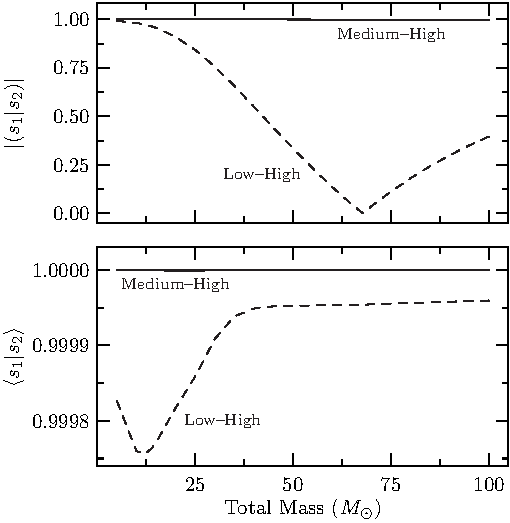
\includegraphics[width=0.55\linewidth]{figures/comparison/Accuracy}
  \end{center}
  \caption[Convergence testing for numerical waveforms ]{
  \label{f:accuracy}
    Convergence testing for numerical waveforms from a
    data-analysis perspective, using the match between waveforms
    computed at different numerical resolutions.  The waveforms are
    scaled to various masses, and the Initial-LIGO noise curve is used
    in the calculation of the match.  The upper panel shows the
    overlap without maximization over arrival time and phase; the
    lower panel shows the overlap after maximization.  In each panel,
    the lower (dashed) line compares the lowest- and
    highest-resolution simulations, while the upper (solid) line
    compares the medium- and highest-resolution simulations.  Note
    that this plot uses only numerical data, with no post-Newtonian
    contribution.}
\end{figure}%
%%%%%%%%%%%%%%%%%%%%%%%%%%%%%%%%%%%%%%%%%%%%%%%%%%%%%%%%%%%%%%%%%%%%%%

Because of the short extent of the numerical waveforms, we need to be
careful when using their Fourier transforms.  The signal can be
corrupted easily by the non-periodicity of the waveforms, and the
discontinuous jumps that result.  For Fig.~\ref{f:accuracy} we
mitigate this problem by increasing the sampling frequency of the
input data, and restricting the Fourier transform to frequencies
corresponding to instantaneous frequencies contained in the data.  The
input data can easily be upsampled in the time domain by interpolating
the phase and amplitude of the complex data to a finer time grid.  We
then perform the transform, and explicitly set the data to zero at
frequencies below $f_{\mathrm{initial}}$ and above
$f_{\mathrm{ringdown}}$, as given in
Eqs.~\ref{eq:MeasuredStartingFreq} and~\ref{eq:MeasuredRingdownFreq}.
While the results do depend on whether or not we impose these cutoffs,
they do not depend sensitively on the actual cutoff frequencies.

The overlap between the lowest- and highest-resolution simulations
(dashed lines) actually passes through zero, as shown in the upper
panel.  Presumably, this is because of loss of phase accuracy over the
course of the simulation.  All three simulations begin with the same
initial data, so the waveforms are most similar at the beginning.
Masses for which this is the most important segment (the lowest
masses) will naturally have the highest overlap between resolutions.
As the simulation progresses, numerical error accumulates---notably in
the phase---so the overlap decreases with masses for which later
segments dominate the overlap (higher masses).  When the overlap is
optimized over arrival time and phase
(sec.~\ref{sec:ihope_match_filter}) we can see that the overlap
becomes much better, as shown in the lower panel, indicating
sufficient accuracy within any frequency band for which phase
coherence is required.  In either case, the medium and highest
resolutions are much more nearly the same.  Without optimization,
their overlap is within a few tenths of a percent of 1; after
optimization, the overlap is within $10^{-6}$ of 1.

In the rest of our analysis we use the highest-resolution waveform.
Because we always optimize over arrival time and phase, the lower
panel of Fig.~\ref{f:accuracy} is the most relevant, and shows that
the waveform has converged to very high accuracy.  The overlaps we
quote below will only be given to three decimal places at most,
because this is roughly the accuracy of the single-precision numerical
methods used in the rest of the chapter.  This accuracy is also
sufficient for searches of gravitational-wave data.  Thus, the
truncation error of the simulated waveform is irrelevant for those
purposes.

Other sources of error include residual eccentricity and spin, the
influence of the outer boundary of the simulation, extrapolation
errors, and coordinate effects, as discussed in Ref.~\cite{Boyle2007}.
The eccentricity had a disproportionately large effect on the error
quoted in that paper because of the matching technique, which is not
used here.  Restricting attention to the other effects of
eccentricity, the uncertainty falls below that due to numerical error.
Similarly, using the techniques of Ref.~\cite{Lovelace2008}, the
initial spins of the black holes have been measured more reliably, and
found to be more than an order of magnitude smaller than previously
determined, allowing us to reduce the estimate for that error to less
than the numerical truncation error.  The various coordinate effects
were all estimated to be of roughly the same magnitude as the
numerical error.

With the numerical error being many times more accurate than needed
for this analysis, and the other sources of uncertainty being of
roughly the same size, these considerations indicate that the overall
error in our fiducial waveform is substantially less than the
precision needed for this analysis.


%%%%%%%%%%%%%%%%%%%%%%%%%%%%%%%%%%%%%%%%%%%%%%%%%%%%%%%%%%%%%%%%%%%%%%
%%%%%%%%%%%%%%%%%%%%%%%%%%%%%%%%%%%%%%%%%%%%%%%%%%%%%%%%%%%%%%%%%%%%%%
\section{Detection efficiency of gravitational-wave templates}
\label{sec:Efficiency} %

We now compare the signal described in the previous section to
restricted, stationary phase \textit{TaylorF2} post-Newtonian
templates with terms up to order 2.0, order 3.5, and a ``pseudo-4.0
pN-order'' term recommended in Ref.~\cite{Pan2007}.  Overlaps are
calculated using the techniques of Sec.~\ref{sec:ihope_match_filter}
with the signal $s$ being the hybrid waveform described in the
previous section, scaled to a range of masses.  We consider both the
Initial- and Advanced-LIGO noise curves.

Plots of the hybrid waveforms in comparison to the Initial-LIGO noise
curve are shown in Fig.~\ref{fig:StildesAndInitialPSD}.
%%%%%%%%%%%%%%%%%%%%%%%%%%%%%%%%%%%%%%%%%%%%%%%%%%%%%%%%%%%%%%%%%%%%%%
\begin{figure}
  \begin{center}
    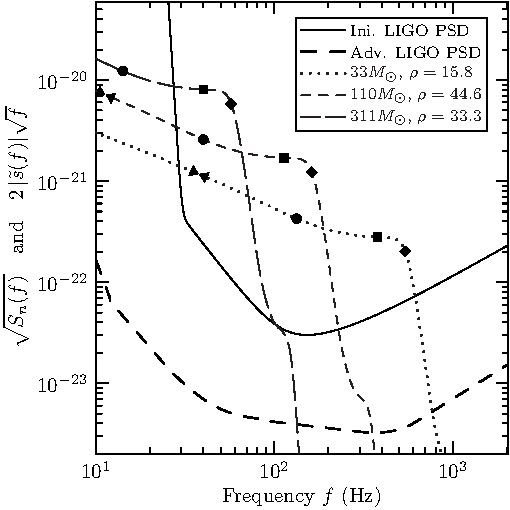
\includegraphics[width=0.55\linewidth]{figures/comparison/StildesAndInitialPSD}
  \end{center}
  \caption[Hybrid Caltech--Cornell waveform scaled to various total masses]{
  \label{fig:StildesAndInitialPSD}
    Hybrid Caltech--Cornell waveform scaled to various total
    masses, with sources optimally oriented and placed at
    \unit[100]{Mpc}, shown against the Initial- and Advanced-LIGO
    noise curves.  Markers are placed along the lines at frequencies
    corresponding to various instantaneous frequencies of the
    waveforms.  The triangles represent the beginning and end of the
    blending region; the circle represents the ISCO frequency; the
    square the light-ring; and the diamond the measured ringdown
    frequency.  See the text for discussion of the normalization.  The
    values given for $\rho$ use the Initial-LIGO noise curve, with
    sources at a distance of 100\,Mpc.}
\end{figure}%
%%%%%%%%%%%%%%%%%%%%%%%%%%%%%%%%%%%%%%%%%%%%%%%%%%%%%%%%%%%%%%%%%%%%%%
The masses are chosen so that various frequencies of interest (the
final stitching frequency, the ISCO, and the ringdown) occur at the
``seismic wall'' for Initial LIGO: \unit[40]{Hz}.  The waveforms
$\tilde{s}$ are scaled to depict the detectability of the signal,
typically quantified by the SNR introduced in
~\eqref{eq:InnerProductSNR}, which may be written as
\begin{equation}
  \label{eq:SNR}
  \rho^{2} \equiv \int_0^\infty \frac{4\, \tilde{s}(f)\,
    \tilde{s}^\ast(f)} {S_n(f)}\, d f = \int_0^\infty
  \frac{\left\lvert 2\, \tilde{s}(f)\, \sqrt{f} \right\rvert^{2}}
  {S_n(f)}\, d\ln{f}\ .
\end{equation}
In the final expression, the numerator and denominator have the same
units, and are directly comparable.  Because the square root of the
denominator is familiar, we plot that along with the square root of
the numerator.  Plotting these two quantities together gives a
graphical impression of the detectability of the waveform, and the
relative importance of each part of the waveform, by its height above
the noise curve.  In Ref.~\cite{BradyCreighton2002}, Brady and
Creighton define a slightly different quantity, the characteristic
strain $h_{\mathrm{char}} \equiv f\, \lvert \tilde{s}(f) \rvert\ .$
The relative factor of $\sqrt{f}$ they use is present so that they can
plot $h_{\mathrm{char}}$ against $\sqrt{f\, S_{n}(f)}$.  Cutler and
Thorne~\cite{Cutler2002} define still another quantity, the signal
strength $\tilde{h}_{s}(f)$, which is related to the Fourier transform
by $\tilde{h}(f) = \sqrt{5}\, \frac{T}{N}\, \tilde{h}(s)\ .$ The
factor of $\sqrt{5}$ comes from averaging over the orientation of the
binary, which we do not do.  $T/N$ is the ratio of the threshold to
the rms noise at the endpoint of signal processing.

\iffalse
\begin{figure}
  % \includegraphics[width=\linewidth]{figures/comparison/AmoebaHistogram}
  \begin{center}
    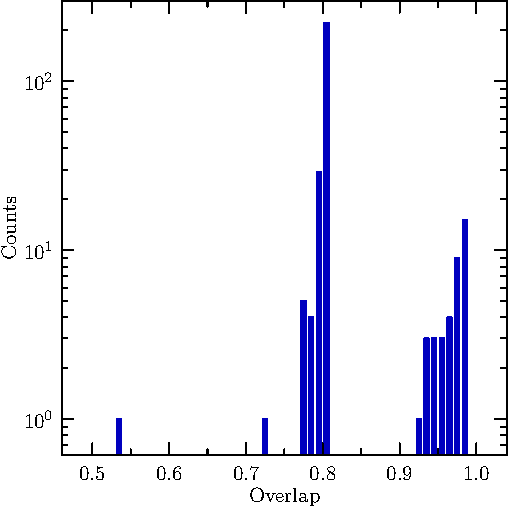
\includegraphics[width=0.55\linewidth]{figures/comparison/Histogram}
  \end{center}
  \caption{Histogram of overlaps found by 300 instances of the Amoeba
    algorithm, optimizing the overlap against a given waveform over
    $M, \eta, f_c$, with randomized initial conditions.  Note the
    logarithmic scale on the vertical axis.  The majority of instances
    produced a lower overlap than the optimum.  We interpret this as
    pointing to the existence of a broad local maximum which did not
    coincide with the global maximum.}
  \label{fig:AmoebaHistogram}
\end{figure}%
\fi

For each template family we initially optimize over signal mass $M$,
symmetric mass ratio $\eta = m_1 m_2 / (m_1 + m_2)^2$, and upper
cutoff frequency $f_c$.  The optimization is performed using a
Nelder--Mead (``amoeba'') algorithm~\cite{numrec_cpp}.  The amoeba
starts with a simplex in the parameter space and proceeds through a
series of steps, each of which will improve the value of the function
at at least one vertex.  The algorithm terminates when all vertices
have converged to the same point to within a specified tolerance.
This process is deterministic, and amounts to an enhanced
steepest-ascent algorithm.  It is therefore only guaranteed to find a
local maximum, and indeed we find that an amoeba instance started at a
random point in the parameter space is most likely to converge to a
point that does not give the highest possible overlap.  We interpret
this as being due to a large region in parameter space containing a
local maximum and a relatively smaller region containing the global
maximum.  We therefore supplement the basic amoeba by running 300
instances with random starting values, and taking the best match
obtained over all instances.  In repeated runs the same optimal
parameters were found by at least some of the amoebas, which supports
the claim that this is the true maximum.

The results of optimizing over all of $M, \eta$ and $f_c$ for selected
masses for Initial LIGO are given in
Table~\ref{tab:ThreeParamOverlapDetailInitial} and summarized in
Fig.~\ref{fig:ThreeParamOverlapSummaries}.  For Initial LIGO, in the
range covered by the current CBC low-mass search $(M < 35
\MSun)$~\cite{Abbott:2008}, the pseudo-4.0 pN \textit{TaylorF2}
waveforms achieve the highest overlaps, exceeding those obtained with
3.5 pN waveforms by $\sim 1\%$.  Above $35 \MSun$ the 3.5 pN waveforms
produce overlaps as much as 4\% greater than those obtained with
pseudo-4.0 pN waveforms over a range from $40$--$80 \MSun$. With the
Advanced-LIGO noise curve, in the CBC low-mass range, the 3.5 pN and
pseudo-4.0 pN waveforms produce overlaps within 2\% of each other,
with 3.5 pN producing higher overlaps below 20 $\MSun$ and pseudo-4.0
pN producing higher overlaps in the range $20$--$35 \MSun$.
Pseudo-4.0 pN continues to give the highest overlaps up to $60 \MSun$,
producing overlaps as much as 4\% greater than those obtained with 3.5
pN waveforms.  Above $60 \MSun$ 3.5 pN waveforms again yield the best
overlaps, by as much as 6\% around 90 $\MSun$.

% We see from Tables~\ref{tab:ThreeParamOverlapDetailInitial}
% and~\ref{tab:ThreeParamOverlapDetail} that the parameters of the
% optimal templates are often far from the parameters of the physical
% waveform, especially for high-mass systems, which emphasize portions
% of the waveform for which the pN and SPA assumptions are poor.  For
% Initial LIGO, pseudo-4.0 pN templates find $M$ to within $19\%$ of
% the true value compared to $52\%$ for 2.0 pN and $159\%$ for 3.5 pN.
% Conversely, for Advanced LIGO, 3.5 pN templates estimate the signal
% mass to within $16\%$ for masses less than $\MSun$, compared to
% $25\%$ for 2.0 pN and $20\%$ for pseudo-4.0 pN templates.

% \Note{Should we drop this paragraph?  We never systematically looked
%   at parameter estimation, and the numbers from the table don't tell
%   a compelling story regarding any of them doing better than the
%   others.}



% \addtolength{\tabcolsep}{3.25mm} \renewcommand{\arraystretch}{1.6}
\begin{table*}
  \begin{center}
    \begin{tabular}{@{}lcccc@{}}
      \hline \hline
      & $(10+10) \MSun$ & $(20+20) \MSun$ & $(30+30) \MSun$ & 
      $(50+50) \MSun$ \\
      \hline
      $\Overlap{s^{\textrm{NR-CC}} |
        h^{\textrm{SPA}_c^{\textrm{ext}}(2.0)}}$ &
      0.99 & 0.98 & 0.97 & 0.96 \\
      $M/\MSun$ &
      $23.27^{+0.13}_{-0.12}$  &
      $25.99^{+0.61}_{-0.56}$  &
      $35.22^{+1.84}_{-1.89}$  &
      $47.52^{+6.87}_{-4.73}$  \\
      $\eta$ &
      $0.199^{+0.0030}_{-0.0030}$  &
      $0.771^{+0.0490}_{-0.0420}$  &
      $1.000_{-0.1390}$  &
      $1.000_{-0.2490}$  \\
      $f_{\mathrm{cut}}$ (Hz) &
      $501.18^{+523.00}_{-153.00}$  &
      $431.35^{+358.00}_{-77.00}$  &
      $296.05^{+53.00}_{-31.00}$  &
      $190.56^{+20.00}_{-14.00}$  \\
      \hline
      $\Overlap{s^{\textrm{NR-CC}} |
        h^{\textrm{SPA}_c^{\textrm{ext}}(3.5)}}$ &
      0.98 & 0.99 & 0.99 & 0.99 \\
      $M/\MSun$ &
      $18.75^{+0.10}_{-0.10}$  &
      $31.88^{+0.77}_{-0.71}$  &
      $47.15^{+4.37}_{-3.27}$  &
      $259.89^{+0.00}_{-194.18}$  \\
      $\eta$ &
      $0.290^{+0.0040}_{-0.0040}$  &
      $0.493^{+0.0530}_{-0.0410}$  &
      $0.756^{+0.2440}_{-0.2290}$  &
      $0.954^{+0.0460}_{-0.2090}$  \\
      $f_{\mathrm{cut}}$ (Hz) &
      $506.50^{+518.00}_{-155.00}$  &
      $448.80^{+576.00}_{-83.00}$  &
      $324.74^{+145.00}_{-42.00}$  &
      $197.17^{+24.00}_{-16.00}$  \\
      \hline
      $\Overlap{s^{\textrm{NR-CC}} |
        h^{\textrm{SPA}_c^{\mathcal{Y}}(4)}}$ &
      0.99 & 0.96 & 0.95 & 0.96 \\
      $M/\MSun$ &
      $23.64^{+0.13}_{-0.12}$  &
      $47.90^{+1.28}_{-1.13}$  &
      $61.81^{+8.68}_{-6.19}$  &
      $89.93^{+20.44}_{-16.60}$  \\
      $\eta$ &
      $0.182^{+0.0030}_{-0.0030}$  &
      $0.181^{+0.0160}_{-0.0140}$  &
      $0.523^{+0.4260}_{-0.1820}$  &
      $0.529^{+0.4720}_{-0.3100}$  \\
      $f_{\mathrm{cut}}$ (Hz) &
      $509.47^{+654.00}_{-145.00}$  &
      $352.44^{+73.00}_{-61.00}$  &
      $309.53^{+72.00}_{-47.00}$  &
      $195.63^{+21.00}_{-15.00}$  \\
      \hline \hline
    \end{tabular}
  \end{center}
  \caption[Overlaps between Caltech--Cornell hybrid waveforms and pN
waveforms in initial LIGO]{
  \label{tab:ThreeParamOverlapDetailInitial}
    Maximum overlaps between Caltech--Cornell hybrid waveforms
    and restricted stationary-phase pN templates using the
    Initial-LIGO noise curve.  The first number in each block is the
    overlap; subsequent numbers are the template parameters that
    achieve this overlap.  Parameter values within the specified
    ranges keep the overlap within 1\% of the maximum by varying that
    parameter, while leaving others fixed.  We restrict the search to
    $0 \leq \eta \leq 1.000$, so the upper error bounds when $\eta\sim
    1.000$ may be artificially small.}
\end{table*}
% \addtolength{\tabcolsep}{-3.25mm} \renewcommand{\arraystretch}{1}

%
% Advanced LIGO results
%

% \addtolength{\tabcolsep}{3.25mm} \renewcommand{\arraystretch}{1.6}
\begin{table*}
  \begin{tabular}{@{}lcccc@{}}
    \hline \hline
    & $(10+10) \MSun$ & $(20+20) \MSun$ & $(30+30) \MSun$ & 
    $(50+50) \MSun$ \\
    \hline
    $\Overlap{s^{\textrm{NR-CC}} |
      h^{\textrm{SPA}_c^{\textrm{ext}}(2.0)}}$ &
    0.98 & 0.92 & 0.91 & 0.94 \\
    $M/\MSun$ &
    $25.15^{+0.02}_{-0.02}$ &
    $47.73^{+0.12}_{-0.11}$ &
    $54.39^{+0.51}_{-0.43}$ &
    $60.19^{+1.55}_{-1.29}$ \\
    $\eta$ &
    $0.170^{+0.0010}_{-0.0010}$ &
    $0.188^{+0.0010}_{-0.0010}$ &
    $0.335^{+0.0080}_{-0.0070}$ &
    $0.891^{+0.0660}_{-0.0490}$ \\
    $f_{\mathrm{cut}}$  (Hz) &
    $444.77^{+132.00}_{-115.00}$ &
    $267.64^{+48.00}_{-50.00}$ &
    $262.44^{+34.00}_{-36.00}$ &
    $182.41^{+24.00}_{-18.00}$ \\
    \hline
    $\Overlap{s^{\textrm{NR-CC}} |
      h^{\textrm{SPA}_c^{\textrm{ext}}(3.5)}}$ &
    0.97 & 0.92 & 0.92 & 0.96 \\
    $M/\MSun$ &
    $20.27^{+0.02}_{-0.02}$ &
    $38.11^{+0.11}_{-0.09}$ &
    $50.09^{+0.49}_{-0.42}$ &
    $78.10^{+1.89}_{-1.50}$ \\
    $\eta$ &
    $0.245^{+0.0010}_{-0.0010}$ &
    $0.277^{+0.0020}_{-0.0020}$ &
    $0.386^{+0.0130}_{-0.0100}$ &
    $0.494^{+0.0760}_{-0.0330}$ \\
    $f_{\mathrm{cut}}$   (Hz) &
    $355.85^{+97.00}_{-88.00}$ &
    $262.83^{+47.00}_{-48.00}$ &
    $281.34^{+41.00}_{-37.00}$ &
    $186.31^{+30.00}_{-19.00}$ \\
    \hline
    $\Overlap{s^{\textrm{NR-CC}} |
      h^{\textrm{SPA}_c^{\mathcal{Y}}(4)}}$ &
    0.97 & 0.96 & 0.94 & 0.90 \\
    $M/\MSun$ &
    $22.24^{+0.02}_{-0.02}$ &
    $46.57^{+0.11}_{-0.11}$ &
    $72.06^{+0.35}_{-0.35}$ &
    $118.50^{+1.99}_{-1.63}$ \\
    $\eta$ &
    $0.208^{+0.0010}_{-0.0010}$ &
    $0.190^{+0.0010}_{-0.0010}$ &
    $0.177^{+0.0020}_{-0.0030}$ &
    $0.186^{+0.0100}_{-0.0070}$ \\
    $f_{\mathrm{cut}}$  (Hz) &
    $473.49^{+551.00}_{-136.00}$ &
    $353.18^{+73.00}_{-69.00}$ &
    $242.43^{+37.00}_{-36.00}$ &
    $152.16^{+19.00}_{-19.00}$ \\
    \hline \hline
  \end{tabular}
  \caption[Overlaps between Caltech--Cornell hybrid waveforms and pN
waveforms in advanced LIGO]{
  \label{tab:ThreeParamOverlapDetail}
    Maximum overlaps between Caltech--Cornell hybrid waveforms
    and restricted stationary-phase pN templates using the
    Advanced-LIGO noise curve.  The first number in each block is the
    overlap; subsequent numbers are the template parameters that
    achieve this overlap.  Parameter values within the specified
    ranges keep the overlap within 1\% of the maximum by varying that
    parameter, while leaving others fixed.  We restrict the search to
    $0 \leq \eta \leq 1.000$, so the upper error bounds when $\eta\sim
    1.000$ may be artificially small.}
\end{table*}
% \addtolength{\tabcolsep}{-3.25mm} \renewcommand{\arraystretch}{1}


A significant feature of
Tables~\ref{tab:ThreeParamOverlapDetailInitial}
and~\ref{tab:ThreeParamOverlapDetail} is the size of the error bars on
the cutoff frequencies.  For $M=20 \MSun$ the cutoff frequency can
vary as much as 128\% above and 28\% below the optimal value while
losing no more than 1\% of overlap. This leads us to consider the
range of possible template parameters which may give high overlaps.
In the next section we consider the reduction in overlap as the
parameters $f_{c}$ and $\eta$ are independently varied from the
optimal value.

\begin{figure}
  % \includegraphics[width=\linewidth]{figures/comparison/ThreeParamOverlapSummary}
  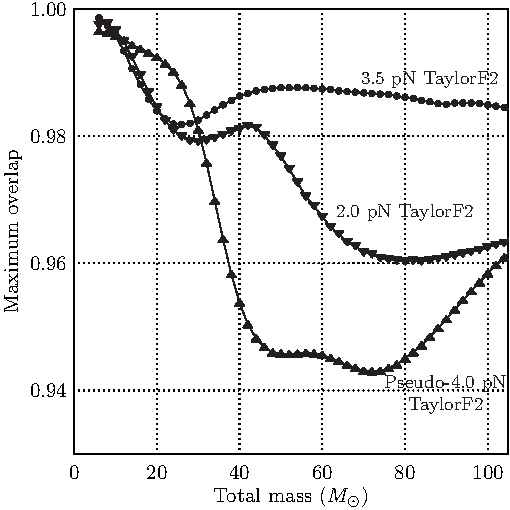
\includegraphics[width=0.5\linewidth]{figures/comparison/ThreeParamOverlapSummaryInitial}
  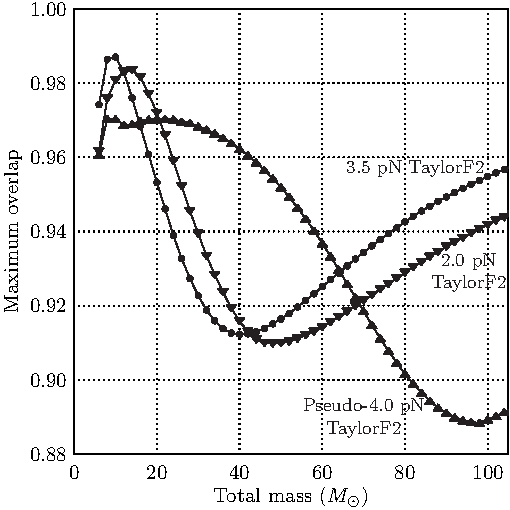
\includegraphics[width=0.5\linewidth]{figures/comparison/ThreeParamOverlapSummaryAdvanced}
  \caption[Overlaps between Caltech--Cornell hybrid waveforms and pN waveforms]{
  \label{fig:ThreeParamOverlapSummaries}
    Left: Overlaps between Caltech--Cornell hybrid waveforms,
    scaled to various masses, and restricted stationary-phase pN
    waveforms for Initial-LIGO PSD. Optimization is over $M$ and
    $\eta$, which the cutoff frequency $f_{c}$ is prescribed by the
    weighted average described below.  The mass ratio $\eta$ is
    allowed to range over unphysical values.  The best-fit values
    found for the pseudo-4.0 pN templates are always physical in this
    case.  See Sec.~\ref{sec:UnrestrictedEta}.  Right: The same, for
    the Advanced-LIGO PSD}
\end{figure}%


\subsection{Effect of upper frequency cutoff}
\label{sec:EffectOfUpperFreqCutoff}

As shown in Fig.~\ref{fig:StildesAndInitialPSD} the amplitude of the
NR waveforms drops sharply at around the lightring frequency, which
depends on the total mass of the binary.  The \textit{TaylorF2}
waveforms do not model the late inspiral, merger or ringdown and hence
will continue to evolve as $f^{-7/6}$ at all frequencies, increasingly
deviating from the NR waveform.  This suggests that the upper
frequency cutoff of the \textit{TaylorF2} waveform should be chosen to
be below the frequency at which the two diverge.  However, the effect
of the divergence is mitigated by the PSD.  The denominator of the
overlap, Eq.~\eqref{eq:OverlapDefinition}, depends on
$\InnerProduct{s|s}$ which is a constant, and $\InnerProduct{h|h}$
which would increase without limit if not for the PSD.
Fig.~\ref{fig:FilterIntegrand} shows $|\tilde{h}(f)|^2/S_n(f)$---the integrand of
$\InnerProduct{h|h}$---for the Initial-LIGO
noise curve for an example \textit{TaylorF2} waveform for an
equal-mass $10\,\MSun$ binary.  We see that above about 450 Hz there
is very little contribution to the integrand, and so extending the
cutoff frequency above this will not impact the overlap.


\begin{figure}
  % \includegraphics[width=\linewidth]{figures/comparison/FilterIntegrand}
  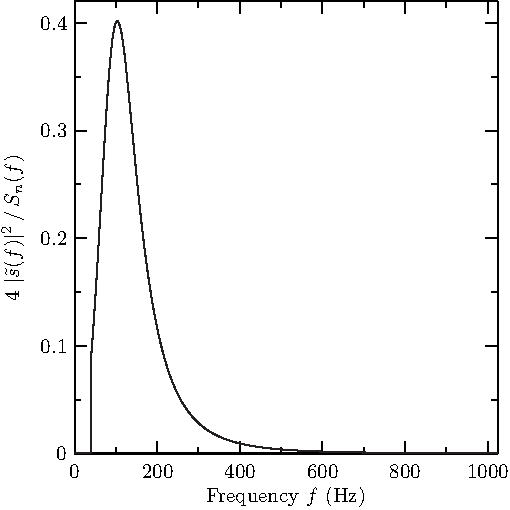
\includegraphics[width=0.50\linewidth]{figures/comparison/Integrand}
  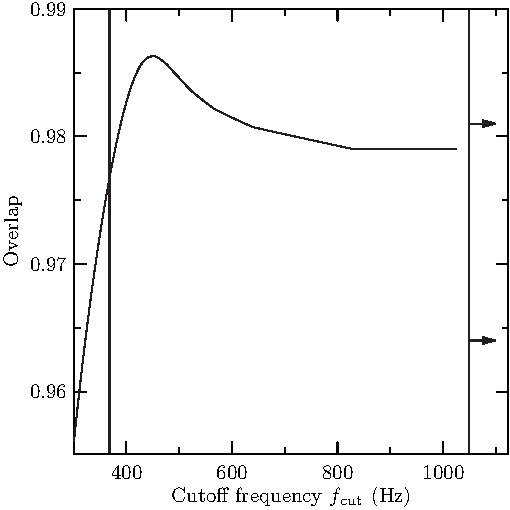
\includegraphics[width=0.50\linewidth]{figures/comparison/Errorbars}
  \caption[Effect of cutoff frequency on overlaps]{
  \label{fig:FilterIntegrand}
    Left: Integrand of Eq.~\eqref{eq:InnerProduct} for a
    \textit{TaylorF2}, 3.5 pN waveform with $M=10$ and $\eta=0.25$, at
    a distance of 100\,Mpc, using the Initial-LIGO noise curve.  Note
    that the shape of this curve does not change as we change $M$ and
    $\eta$; only the vertical scale changes.  Right: Overlap between
    Caltech--Cornell waveform scaled to $M=40\,\MSun$ and restricted
    \textit{TaylorF2}, 3.5 pN waveform using the best-match values for
    $M$ and $\eta$, as a function of the cutoff frequency $f_c$, with
    the Initial-LIGO noise curve.  The vertical bars are meant to
    delineate 1\% loss.  Note that the upper bound extends to higher
    frequencies indefinitely.  }
\end{figure}%


The numerator of the overlap, $\InnerProduct{s|h}$, can only increase
as the cutoff frequency is raised, however frequencies above the
lightring where the waveforms have diverged will contribute very
little.  The effect of including higher frequencies on the overlap is
therefore determined by the $\InnerProduct{h|h}$ term in the
denominator.  For systems with ringdown frequencies well above the
peak of the integrand in Fig.~\ref{fig:FilterIntegrand}, this term
will not significantly reduce the overlap.  For example, binaries of
total mass roughly $40\,\MSun$ have ringdown frequencies at roughly
450\,Hz.  Only a small fraction of the SNR comes from higher
frequencies.  Thus, we expect that systems with lower masses should
not suffer great loss in overlap if the cutoff frequency is higher
than ringdown.  However for higher-mass systems the overlap can be
significantly reduced if the upper frequency cutoff is too large.
This is indeed what we find, as shown by a representative example on
the right in Fig.~\ref{fig:FilterIntegrand}.  For this $40\,\MSun$
system, using the Initial-LIGO noise curve, the optimal cutoff
frequency is around 450\,Hz---roughly the ringdown frequency.
Decreasing the cutoff quickly decreases the overlap.  The cutoff may
be increased almost indefinitely, however, with only 0.5\% loss in
overlap.  This, of course, changes when using the Advanced-LIGO noise
curve.  We revisit this issue in Sec.~\ref{sec:Recommendations}.


\subsection{Unrestricted $\eta$}
\label{sec:UnrestrictedEta}

The physical symmetric mass ratio is restricted to the range $0 < \eta
\leq 0.25$, values above this imply complex-valued masses.  However
the pN waveforms are well-behaved for $0 < \eta < 1.0$, and as seen
from Tables~\ref{tab:ThreeParamOverlapDetailInitial}
and~\ref{tab:ThreeParamOverlapDetail}, the highest overlaps are often
obtained at unphysical values of $\eta$.  In
Fig.~\ref{fig:PhysicalEta} we show the effect of limiting the
optimization to physical $\eta$.  At high masses, the limitation
reduces the optimal overlap by up to 12\%.  \textit{TaylorF2}
waveforms with $\eta \leq 1/4$ would not be expected to accurately
model the late-inspiral and merger part of the waveform, as
non-Newtonian effects are increasingly significant in this region.  We
find that allowing unphysical $\eta$ broadens the space of waveforms
covered by the \textit{TaylorF2} approximation sufficiently to capture
more of the late-inspiral and merger.

\begin{figure}
  % \includegraphics[width=\linewidth]{figures/comparison/PhysicalEta}
  \begin{center}
    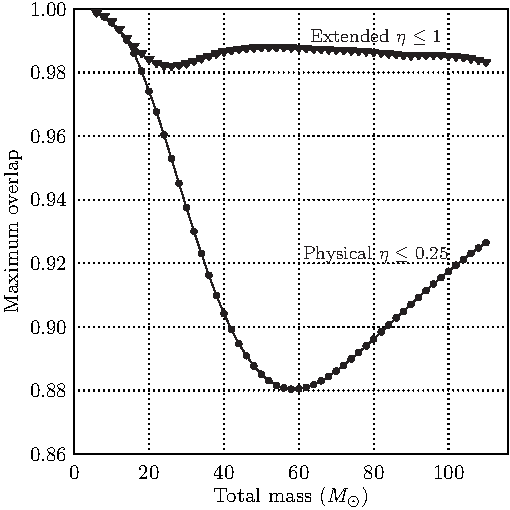
\includegraphics[width=0.55\linewidth]{figures/comparison/PhysicalAndUnphysicalEta}
  \end{center}
  \caption[Maximum overlaps obtained by allowing $\eta$ to range over unphysical values]{
  \label{fig:PhysicalEta}
    Maximum overlaps obtained by allowing $\eta$ to range over
    unphysical values, compared to those obtained by restricting the
    range of $\eta$.  These overlaps are generated using 3.5 pN
    TaylorF2 templates, searching over values of the total mass and
    mass ratio.  Extending to unphysical values of $\eta$ improves the
    match by up to 11\%.}
\end{figure}%


%%%%%%%%%%%%%%%%%%%%%%%%%%%%%%%%%%%%%%%%%%%%%%%%%%%%%%%%%%%%%%%%%%%%%%
%%%%%%%%%%%%%%%%%%%%%%%%%%%%%%%%%%%%%%%%%%%%%%%%%%%%%%%%%%%%%%%%%%%%%%
\section{Recommendations for improvements}
\label{sec:Recommendations} %

Based on the analysis of the previous sections we propose a series of
adjustments to searches using \textit{TaylorF2} template waveforms to
enhance the efficiency of those searches.  First, as seen in
Fig.~\ref{fig:ThreeParamOverlapSummaries} for Initial LIGO, adding
terms up to 3.5 pN order produces overlaps as large or larger than the
current 2.0 pN templates over most of the mass range, while the
pseudo-4.0 pN templates recommended in Ref.~\cite{Pan2007} produce
slightly larger overlaps at masses near $20\,\MSun$.  Thus, we
recommend pseudo-4.0 pN templates for the low mass range, $M < 35
\MSun$, and 3.5 pN templates for higher masses.  The improvement due
to 3.5 pN templates over 2.0 pN generally holds for Advanced LIGO as
well.  The 3.5 pN templates produce larger overlaps than 2.0 pN
templates above $50\,\MSun$ without a significant loss (within 1\%) at
lower masses.  However, there is a large region for which the
pseudo-4.0 pN term does significantly better.  When using an
Advanced-LIGO noise curve, we recommend 3.5 pN templates generally,
2.0 pN templates in the range $12$--$21\,\MSun$ and pseudo-4.0 pN
templates for masses in the range $21$--$65\,\MSun$.

As a second improvement, we note from Fig.~\ref{fig:PhysicalEta} that
allowing $\eta$ to range over unphysical values significantly improves
matches with 3.5 pN templates above $30\,\MSun$. In preliminary
studies we have found that extending to $\eta \leq 1$ roughly doubles
the size of the template bank, and the advantages must therefore be
weighed against the increase in false alarm rate.

\begin{figure}
  % \includegraphics[width=\linewidth]{figures/comparison/FcRecommendationInit}
  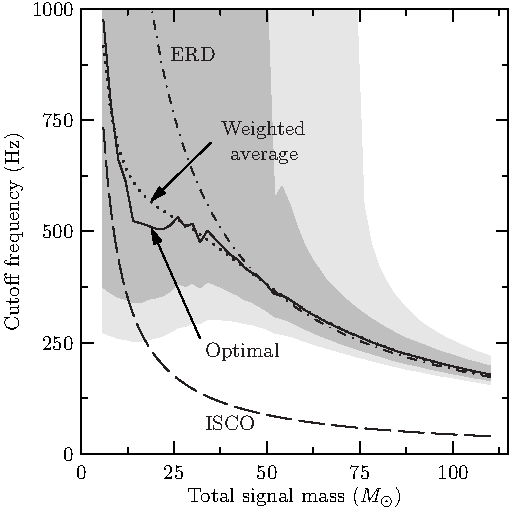
\includegraphics[width=0.5\linewidth]{figures/comparison/FcRecommendationInitial}
  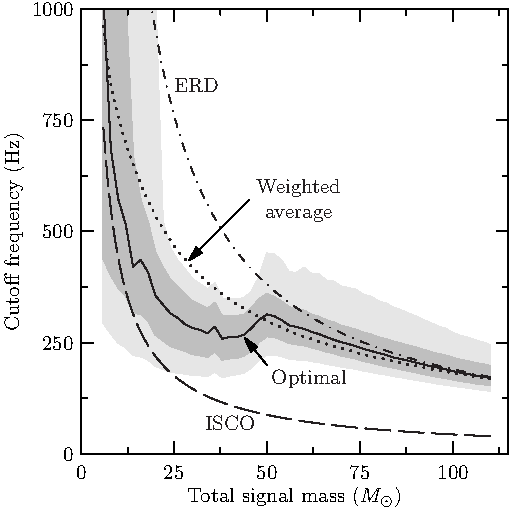
\includegraphics[width=0.5\linewidth]{figures/comparison/FcRecommendationAdvanced}
  \caption[Recommended cutoff frequencies]{
  \label{fig:FcRecomendations}
    Left: Candidate $f_c$ values for 3.5 pN templates with
    Initial LIGO.  The dark gray band contains cutoff frequencies with
    matches within 1\% of the value at which the best overlap was
    obtained.  The light gray band contains frequencies with matches
    within 3\%.  Right: Candidate $f_c$ values for 3.5 pN templates
    with Advanced LIGO.  The dark gray band contains cutoff
    frequencies with matches within 1\% of the value at which the best
    overlap was obtained.  The light gray band contains frequencies
    with matches within 3\%.  Note that the weighted-average cutoff
    extends past the 1\% error bars for $12 < M/\MSun < 40$.  However,
    in that same region, the 3.5 pN templates do poorly overall, and
    we recommend pseudo-4.0 pN templates.  The optimal cutoff
    frequency for pseudo-4.0 pN templates is much closer to the
    weighted-average cutoff in this mass range.}
\end{figure}%

Our third recommendation involves the cutoff frequency used for the
template waveform.  Optimization over the cutoff frequency is too
computationally intensive to be done in searches.  Currently, the
cutoff frequency is typically taken to be the Schwarzschild ISCO
frequency.  To examine the effect of this choice we vary $f_c$ while
keeping the mass and $\eta$ at their optimal values, for each of the
signal masses in our range.  The result of one such variation is shown
in Fig.~\ref{fig:FilterIntegrand} (right).
Figs.~\ref{fig:FcRecomendations} shows the variations for all masses,
highlighting the regions within which the overlap drops by less than
1\% (dark gray) and 3\% (light gray) of the optimal value.  This
figure also shows the ISCO and ERD frequencies, neither of which stays
within the 1\% band for both Initial and Advanced LIGO.  In
particular, the ISCO is a poor choice for both Initial and Advanced
LIGO except at very low masses, where the precise value of the cutoff
is almost irrelevant.

The ISCO is often pointed to---somewhat arbitrarily---as a good
estimate of the breakdown of post-Newtonian
approximations~\cite{Blanchet2006}.  So, for instance, if we were to
match a pN template to a physical waveform, beginning at some point in
the distant past, we might expect them to separate quite badly near
the ISCO.  Of course, for realistic black-hole binaries, the
gravitational waves will only enter the LIGO band late in the
inspiral---just before the ISCO for low-mass systems, or after the
ISCO for high-mass systems.  We can see from
Fig.~\ref{fig:StildesAndInitialPSD} that, for masses below about
$30\,\MSun$, the ISCO is high enough that lower-frequency parts of the
waveform contribute the most to the SNR.  For very high masses,
however, this basically cuts the waveform down to nothing.  In Initial
LIGO, the ISCO is completely buried in seismic noise for masses above
about $100\,\MSun$.  Thus, we must move the cutoff frequency up.  We
cannot push the cutoff far above ringdown, because the physical
waveform simply ceases to exist (see
Fig.~\ref{fig:StildesAndInitialPSD}).  It has been suggested that an
``effective ringdown'' (ERD) frequency $f_{\mathrm{ERD}} \equiv 1.07\,
f_{\mathrm{Ringdown}}$ is a useful upper limit~\cite{Pan2007}.  For
intermediate masses, we would like to interpolate somehow between
these two extremes of ISCO and ERD.  We suggest setting the cutoff
frequency to a weighted average of the two, where the weights are the
contributions to the SNR below the given frequency.  If we assume
coherent phasing between the template and the physical waveform, we
can simply take the amplitudes of the two waveforms.  Also, note that
the restricted SPA approximation for the amplitude is reasonable.
Thus, define
\begin{eqnarray}
  \label{eq:rhoISCO}
  \rho_{\mathrm{ISCO}}^{2} &\equiv & \int_{0}^{f_{\mathrm{ISCO}}}\,
  \frac{f^{-7/3}}{S_{n}(f)}\, d f\ , \\
  \label{eq:rhoERD}
  \rho_{\mathrm{ERD}}^{2} &\equiv & \int_{f_{\mathrm{ISCO}}}^{f_{\mathrm{ERD}}}\,
  \frac{f^{-7/3}}{S_{n}(f)}\, d f\ , \\
  \label{eq:rhoTOT}
  \rho_{\mathrm{tot}}^{2} &\equiv & \int_{0}^{f_{\mathrm{ERD}}}\,
  \frac{f^{-7/3}}{S_{n}(f)}\, d f\ , \\
  \label{eq:fCut}
  f_{\mathrm{cut}} &\equiv & \frac{f_{\mathrm{ISCO}}\ \rho_{\mathrm{ISCO}} +
    f_{\mathrm{ERD}}\ \rho_{\mathrm{ERD}}} {\rho_{\mathrm{tot}}}\ .
\end{eqnarray}
We have already dropped constant factors in the expressions for $\rho$
that will cancel out.

Note that these expressions only depend on the total mass by way of
the limits of integrations---which are very simple, known functions of
the mass---so these integrals could be done just once for a given
noise curve, storing the intermediate values.  When the cutoff needs
to be calculated, the cumulative integral could be evaluated at the
given ISCO and ringdown frequencies.  Hence, this would be a fast way
of calculating the cutoff, with no need to do the integrals each time
the cutoff is needed.

We can test this recommended frequency by comparing it to the optimal
cutoff frequency found by the amoeba search described in
Sec.~\ref{sec:Efficiency}.  For 3.5 pN templates in Initial LIGO, we
find that it is an excellent match to the optimal frequency.
Fig.~\ref{fig:FcRecomendations} shows these two values, along with
dark and light bands showing the regions in which changing $f_{c}$
results in a loss of overlap of 1\% and 3\%, respectively.  Of course,
the same figure shows that using the ERD recommendation would stay
within the 1\% error bounds.  Nonetheless, the close match between
this recommendation and the true optimum suggests that it is sound.
Thus, our final recommendation is to use the weighted-average
frequency cutoff throughout the entire mass range.  While our analysis
has been restricted to equal-mass systems, the cutoff frequency we
have defined here could be applied to unequal-mass systems as well.
It will be interesting to see how this cutoff fares in those
situations.

Similar results hold for Advanced LIGO, when using our recommended
template for each mass.  That is, in regions where 3.5 pN templates do
poorly (see Fig.~\ref{fig:ThreeParamOverlapSummaries}), the weighted
average is a poor predictor of the optimal cutoff frequency using
those templates, as shown in Fig.~\ref{fig:FcRecomendations}.
However, in those same regions---where pseudo-4.0 pN templates do
well---the weighted average is a good predictor of the optimal cutoff
frequency for 4.0 pN templates.  Thus, again, we recommend using the
weighted-average frequency cutoff throughout the entire mass range
with Advanced LIGO.

By prescribing a cutoff frequency, the search does not need to extend
over that parameter.  Similarly, by prescribing a post-Newtonian
order, we need use only one template for a given total mass.  On the
other hand, if these recommendations decrease the overlap found by too
much when using them compared to the overlap found by an unconstrained
search, it may be better to search the larger parameter space.  We can
evaluate the loss in overlap by comparing the results found using our
recommendations to the results found when searching over the set of
all three template families, and all masses, mass ratios, and cutoff
frequencies.  We have determined that this loss in overlap when using
our recommendations is always less than 0.0025 for Initial LIGO, and
less than 0.007 for Advanced LIGO.

\iffalse
\begin{figure}
  \begin{center}
    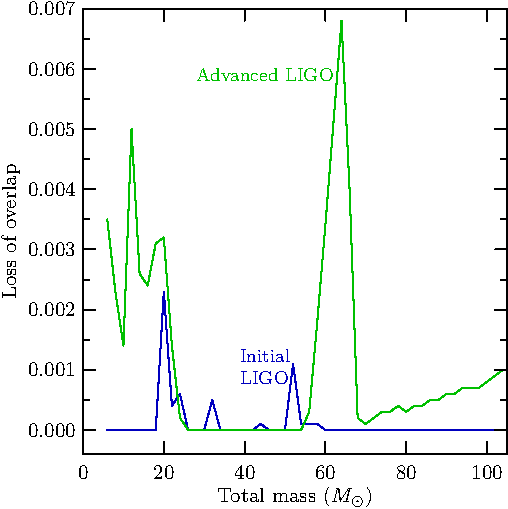
\includegraphics[width=0.55\linewidth]{figures/comparison/WeightedAverageLoss}
  \end{center}
  \caption{Loss in overlap when using our recommendations, compared to
    results searching over all template families, masses, mass ratios,
    and cutoff frequencies.  Our recommendations prescribe the
    template family for a given total mass and the cutoff frequency to
    be used.  In that case, the search is performed for the optimal
    mass and mass ratio of the template.  For Initial LIGO, the loss
    in overlap when using our recommendations is always less than
    0.0025; for Advanced LIGO the loss is always less than 0.007.}
  \label{fig:WeightedAverageLoss}
\end{figure}%
\fi

\section{Conclusions}
\label{sec:Conclusions} %

We have compared high-accuracy NR waveforms for equal-mass binary
black holes from the Caltech--Cornell group to stationary phase
post-Newtonian waveforms.  We examined a number of factors that
influence the matches between the two, with the goal of optimizing the
matches and hence improving the efficiency of templated searches in
Initial and Advanced LIGO.  We first considered the effect of the
post-Newtonian order to which the phase evolution is taken, and found
that adding terms up to 3.5 pN or pseudo-4.0 pN to the currently-used
2.0 pN templates significantly improves the matches over a large range
of masses, as shown in Fig.~\ref{fig:ThreeParamOverlapSummaries}.  We
then studied the effect of varying the upper cutoff frequency of the
templates.  The frequency that achieves the optimal match is a
function of mass, and we find this function is well-approximated by an
average between ISCO and ERD, weighted by contribution to the SNR, as
shown in Fig.~\ref{fig:FcRecomendations}.  Finally, we allow the
symmetric mass ratio $\eta$ to range over unphysical values up to
$1.0$, and find that this dramatically improves matches, as shown in
Fig.~\ref{fig:PhysicalEta}.  Based on the results we recommend
adjusting the searches using \textit{TaylorF2} template waveforms by
going up to 3.5 pN or 4.0 pN over most of the mass range, integrating
up to our recommended cutoff, and allowing allowing $\eta$ to extend
up to 1.  For Initial LIGO, the overlaps obtained using these
parameters is always within 0.0025 of overlaps achievable by
optimizing over all three parameters.

In future work we plan to extend this analysis to unequal-mass and
spinning black-hole systems.  We have found that allowing unphysical
values of $\eta$ roughly doubles the size of the template bank, and we
also plan to study the impact of this on the false alarm rate.


